\documentclass[12pt,a4paper]{scrartcl}
\usepackage[utf8]{inputenc}
\usepackage[english,russian]{babel}
\usepackage{indentfirst}
\usepackage{misccorr}
\usepackage{graphicx}
\usepackage{amsmath}
\usepackage{multirow}
\usepackage{pgfplots}
\usepackage[top=1cm, bottom=1cm, left=1cm, right=1cm]{geometry}
\pgfplotsset{compat=1.9}

\begin{document}
	\graphicspath{{/home/cd7567/Pictures/TeXImgs}}
	
	\newcommand{\ms}{\mathstrut}
	\newcommand{\msp}{\hspace{0.5cm}}
	\newcommand{\al}{\alpha}
	\newcommand{\dg}{^\circ}
	\newcommand{\qd}[2]{^{\frac{#1}{#2}}}
	\newcommand{\qdm}[2]{^{-\frac{#1}{#2}}}
	\newcommand{\lm}[2]{\underset{#1 \rightarrow #2}{\lim}}
	\newcommand{\sfrac}[2]{\dfrac{\strut #1}{\strut #2}}
	\newcommand{\equal}[1]{\overset{(#1)}{=}}
	\newcommand{\linevdots}{\ \raisebox{-.08\height}{\vdots}\ }
	\newcommand{\linecvdots}{\ \raisebox{-.08\height}{\vdots}\hspace{-0.13cm}\raisebox{.15\height}{\cancel{\phantom{a}}\hspace{0.06cm}}}
	\newcommand{\combox}[1]{\ms \msp \msp \begin{minipage}{0.95\linewidth}
			#1
	\end{minipage}}
	
	\newtheorem{pr}{Задача}
	\newtheorem{ex}{Пример}
	\newtheorem{dfn}{Def}
	\newtheorem{theorem}{Th}
	
	\newenvironment{slv}{\ms \msp \textit{Решение:}}{}
	\newenvironment{proof}{\ms \msp \textit{Доказательство: }}{\hfill $\square$}
	
	\begin{titlepage}
		
		\vspace*{\fill}
		
		\begin{center}
			
\includegraphics[scale=0.8]{MIPT.png}
			\\[0.7cm]\Huge Московский Физико-Технический Институт\\(национальный исследовательский университет)
			\\[2cm]\LARGE Отчет по эксперименту
			\\[0.5cm]\noindent\rule{\textwidth}{1pt}
			\\\Huge\textbf{Современные средства\\получения и измерения вакуума}
			\\[-0.5cm]\noindent\rule{\textwidth}{1pt}
		\end{center}
		
		\begin{flushleft}
			\textit{Работа №2.3.1; дата: 11.10.21}\hfill\textit{Семестр: 2}
		\end{flushleft}
		
		\vspace*{\fill}
		
		\begin{flushleft}
			Выполнил: \hspace{\fill} Группа:
			\\Кошелев Александр \hspace{\fill} Б05-105
		\end{flushleft}
	\end{titlepage}
	
	%Страница 2
	
	\begin{flushleft}
		\footnotesize{Современные средства получения и измерения вакуума} \hspace{\fill} \footnotesize{2}
		\\[-0.3cm]\noindent\rule{\textwidth}{0.3pt}
	\end{flushleft}
	
	\section{Аннотация}
	
	\textbf{Цель работы: }
	\begin{enumerate}
		\item Измерение объемов форваккумной и высоковакуумной частей установки
		\item Определение скорости откачки системы
	\end{enumerate}
	
	\textbf{Схема установки:}
	\begin{center}
		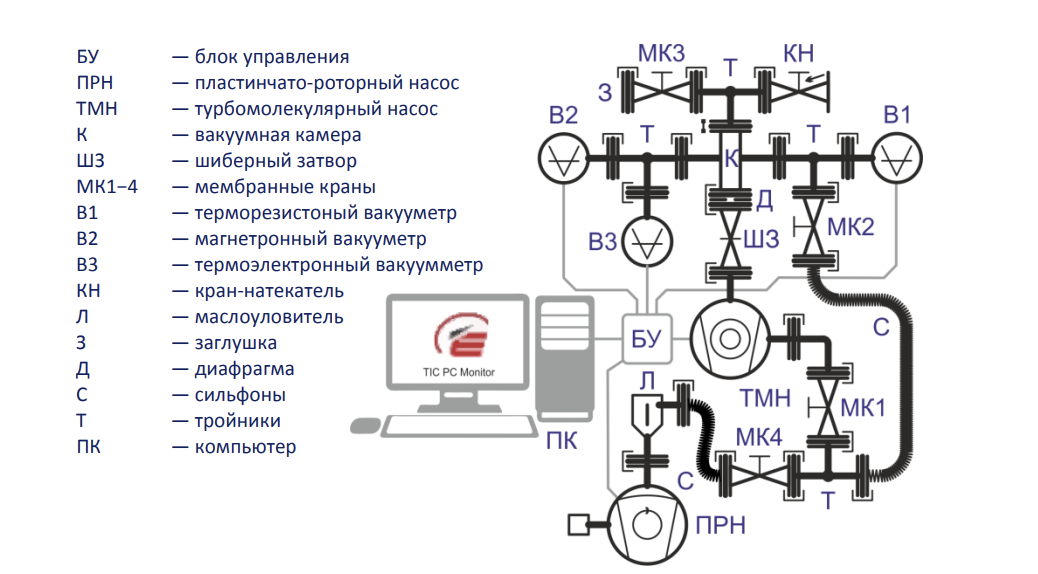
\includegraphics[scale=0.3]{PIC_1.png}
		\\\textbf{Рис. 1:} Схема установки
	\end{center}
	
	\textbf{В работе используются:}
	вакуумная установка с форвакуумным пластинчато-роторным насосом и турбомолекулярным насосом для достижения высокого вакуума. Используются параллельно терморезисторный, термоэлектронный и магнетронный вакуумметры.
	
	\section{Теоретические сведения}
	
	Одна из основных характеристик систем, работающих при вакууме -- число Кнудсена:
	
	\begin{equation}
	Kn = \frac{\lambda}{d}, 
	\end{equation}
	
	$\lambda$ -- длина свободного пробега молекул газа, $d$ -- характерный размер системы.
	
	\medskip
	В зависимости от значений числа Кнудсена определяют:
	\begin{enumerate}
		\item низкий вакуум -- $Kn \ll 1$
		\item средний вакуум -- $Kn \sim 1$
		\item высокий вакуум -- $Kn \gg 1$
	\end{enumerate}
	
	Выпишем основные формулы, отображающие теоретические зависимости между исследуемыми величинами.
	
	Скорость откачки:
	\begin{equation}
	S = \frac{dV}{dt};
	\end{equation}	
	
	Падение давления:
	\begin{equation}
	\Delta P = P_{\text{вх}} - P_{\text{вых}};
	\end{equation}
	
	Пропускная способность:
	\begin{equation}
	U = \frac{Q}{\Delta P};
	\end{equation}
	
	%Страница 3
	
	\newpage
	
	\begin{flushleft}
		\footnotesize{Современные средства получения и измерения вакуума} \hspace{\fill} \footnotesize{3}
		\\[-0.3cm]\noindent\rule{\textwidth}{0.3pt}
	\end{flushleft}
	
	Основное уравнение вакуумной механики:
	\begin{equation}
	\frac{1}{S_{0}} = \frac{1}{S_{text{н}}} + \frac{1}{U};
	\end{equation} 
	
	\begin{equation}
	Q_{\text{н}} = V\frac{P_{\text{к}} - P_{\text{н}}}{\Delta t}		
	\end{equation}
	
	Проводимость отверстия:
	\begin{equation}
	U_{\text{отв}} = \frac{1}{4} \pi R^{2} \sqrt{\frac{8kT}{\pi m}} \sim R^{2}\sqrt{T/m}
	\end{equation}
	
	Проводимость длинного трубопровода
	\begin{equation}
	U_{\text{тр}} = \frac{4}{3} \frac{R^{3}}{L} \sqrt{\frac{2\pi kT}{m}} \sim \frac{R^{3}}{L} \sqrt{\frac{T}{m}} 
	\end{equation}
	
	Уравнение откачки газа
	\begin{equation}
	P\left( t \right) = P_{1}\exp \left(- \frac{S_{0}}{V_{0}}t \right)
	\end{equation}
	
	\section{Проведение эксперимента}
	
	\paragraph{Определение объемов частей установки} \hfill
	
	\par Введем обозначения: $p_1$ -- давление в установке сразу после откачки ТМН, $p_2$ -- давление в вакуумной камере после выравнивания с сильфоном, $p_3$ -- давление в вакуумной камере после выравнивания с объемом ТМН, $V_{\text{сильф}} = 265\, \mathrm{ml}$ -- объем сильфона, $V_{\text{к}}$ -- объем ваккумной камеры, $V_{\text{тмн}}$ -- суммарный объем вакуумной магистрали и рабочего объема ТМН.
	
	Теперь при помощи закона Бойля-Мариотта можем вывести связи объемов частей установки:
	
	\begin{equation*}
	V_{\text{к}} = \sfrac{p_{\text{атм}} - p_2}{p_2 - p_1}V_{\text{сильф}}
	\ \ \ \ \ \ \ \ \ \ \ \ \ \ \ \ \ \ \ \ 
	V_{\text{тмн}} = \sfrac{p_{\text{2}} - p_3}{p_3 - p_1}(V_{\text{сильф}} + V_{\text{к}})
	\end{equation*} 
	
	Давление в установке $170$ mbar, давление камеры $220$ mbar, а значит объем камеры:
	$$V_{\text{к}} = (0.84 \pm 0.05)\ \mathrm{l} $$\\
	Объем установки: $$ V_0 = (1.26 \pm 0.05)\ \mathrm{l} $$.\\
	
	\paragraph{Определение эффективной скорости откачки форвакуумным насосом} \hfill \\
	По причине большого объема данных здесь таблицу приводить не станем. Построим график зависимости $\ln \frac{P}{P_0}(t)$ в области, где эта зависимость близка к линейной.
	
	Согласно формуле 9:
	$$P = P_0 \exp \left(\sfrac{S_0}{V_0}t\right) \Rightarrow \ln \sfrac{P}{P_0} = -\sfrac{S_0}{V_0}t = -\sfrac{t}{\tau}$$
	
	%Страница 5
	
	\newpage
	
	\begin{flushleft}
		\footnotesize{Современные средства получения и измерения вакуума} \hspace{\fill} \footnotesize{5}
		\\[-0.3cm]\noindent\rule{\textwidth}{0.3pt}
	\end{flushleft}
	
	\begin{center}
		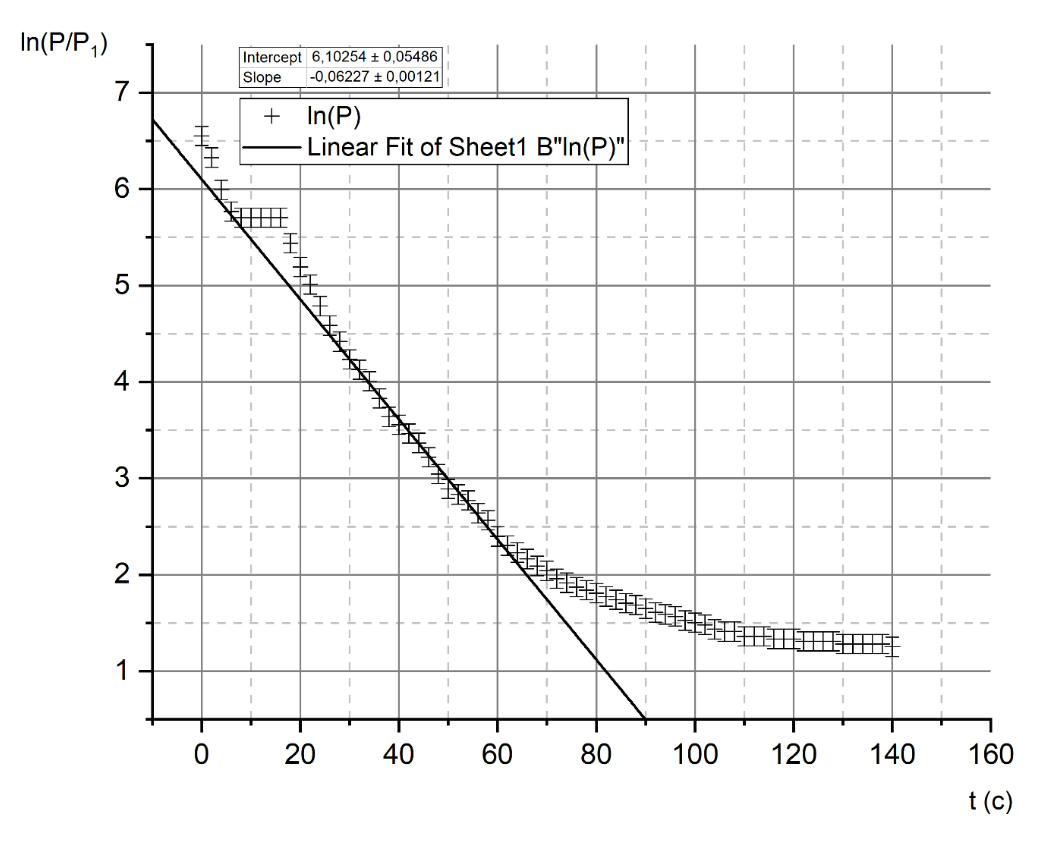
\includegraphics[scale = 0.4]{PIC_2.png}
		\\\textbf{Рис. 2:} График зависимости $\ln \frac{P}{P_0}(t)$
	\end{center}
	
	Вычислим эффективную скорость форвакуумной откачки. Для этого требуется найти коэффициент наклона графика. На интервале, где зависимость можно считать линейной. Таким образом получим:
	$$ \tau = \sfrac{t}{\ln(P / P_0)} = (16.06 \pm 0.02 ) \; \mathrm{s} $$
	Отсюда найдём скорость откачки форвакуумным насосом:
	$$ S = (0.25 \pm 0.05) \; \sfrac{\mathrm{m}^3 }{\mathrm{s}}$$
	
	
	\paragraph{Определение эффективной скорости откачки турбомолекулярным насосом} \hfill
	
	Приведем аналогичный предыдущему пункту график:
	
	\begin{center}
		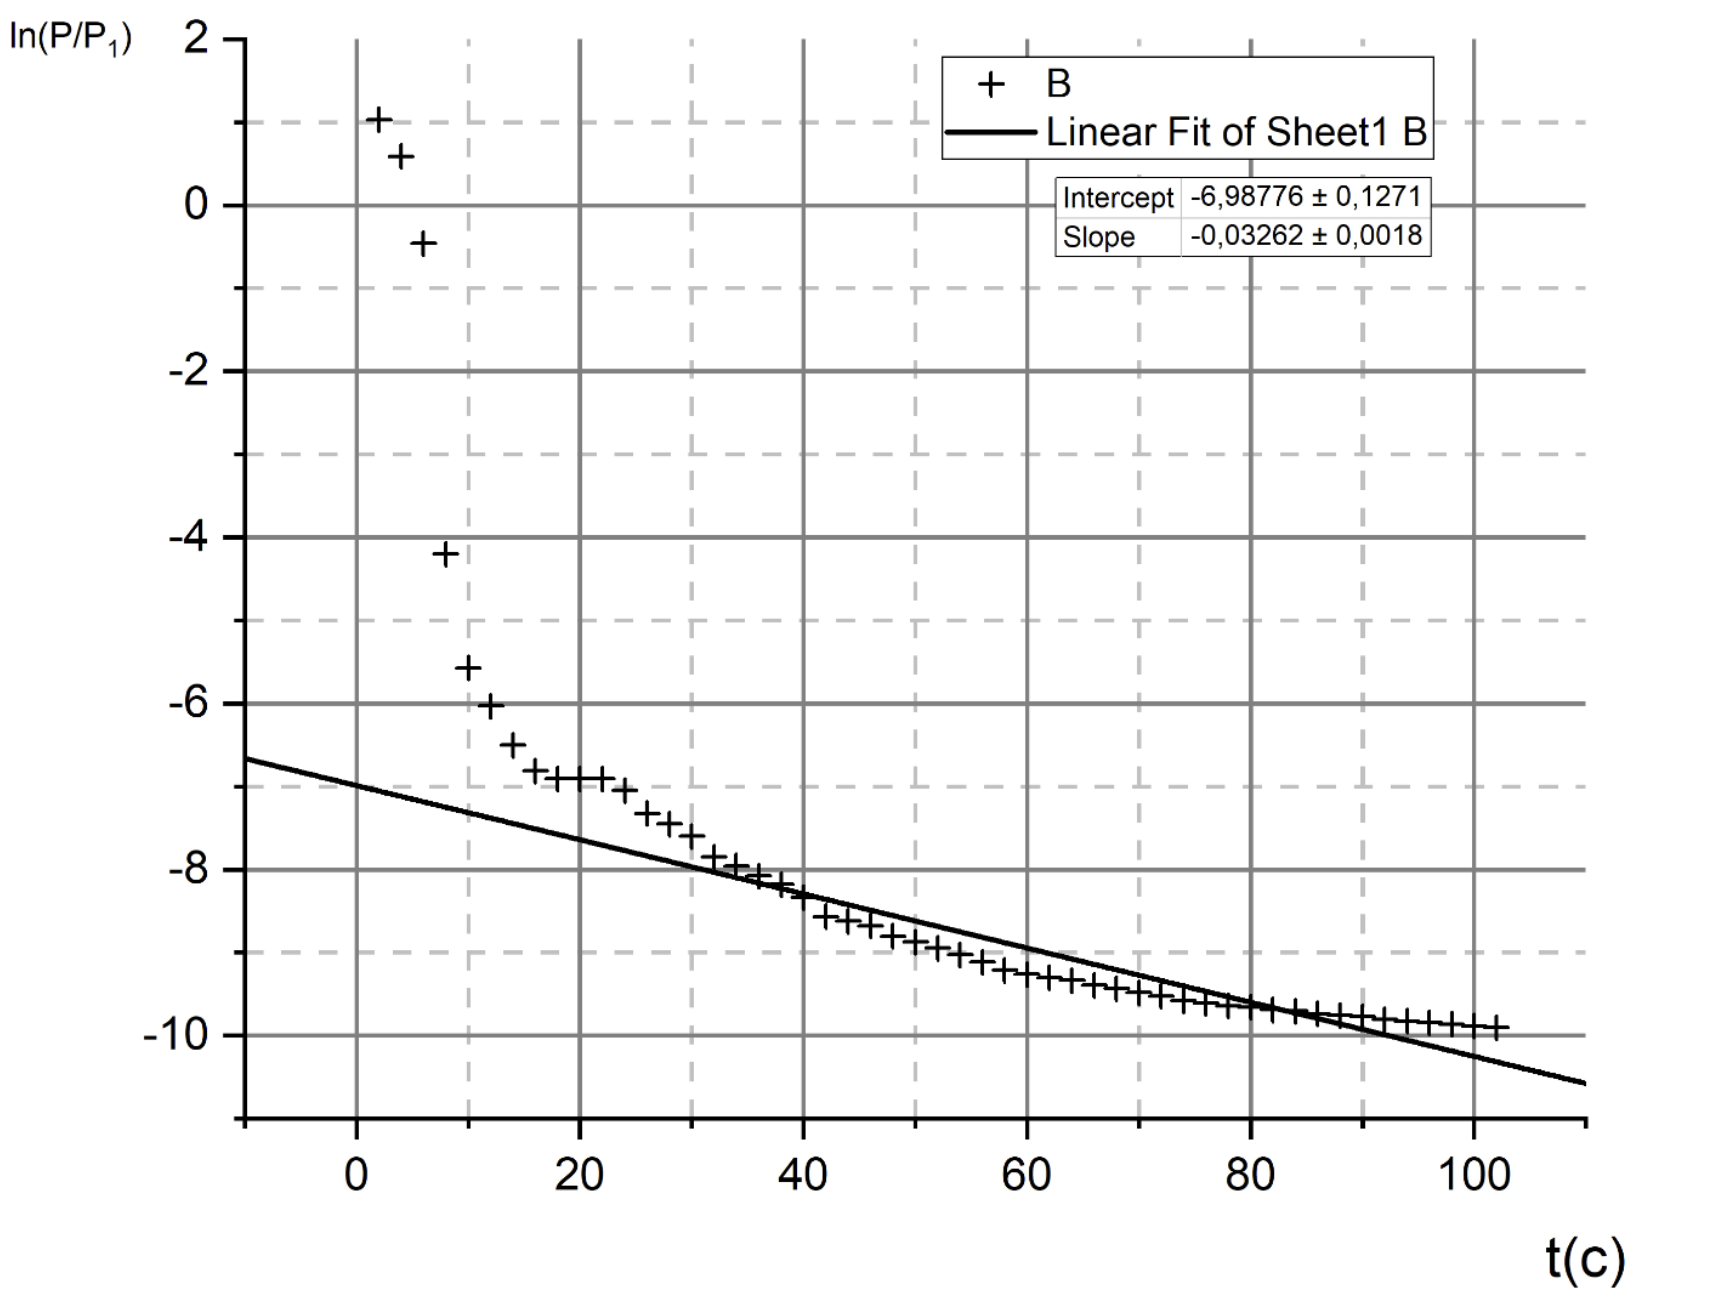
\includegraphics[scale=0.2]{PIC_3.png}
		\\\textbf{Рис. 3:} График зависимости $\ln \frac{P}{P_0}(t)$
	\end{center}
	
	%Страница 6
	
	\newpage
	
	\begin{flushleft}
		\footnotesize{Современные средства получения и измерения вакуума} \hspace{\fill} \footnotesize{6}
		\\[-0.3cm]\noindent\rule{\textwidth}{0.3pt}
	\end{flushleft}
	
	Из графика зависимости получаем $\tau$:
	$$\tau = 0.049\ \text{s}$$
	
	Отсюда найдём скорость откачки турбомолекулярным насосом:
	$$ S = 49 \; \sfrac{\mathrm{l} }{\mathrm{s}}$$
	
	\section{Вывод}
	\begin{enumerate}
		\item В результате выполнения данной работы, был получен вакуум $P \sim 10^{-5} $ торр.
		\item Определена скорость откачки форвакуумным насосом $ S = (0.25 \pm 0.05) \; \sfrac{\mathrm{m}^3 }{\mathrm{s}}$
		\item Определена скорость откачки турбомолекулярным насосом $ S = 49 \; \sfrac{\mathrm{l} }{\mathrm{s}}$
	\end{enumerate}
\end{document} 	